\documentclass[12pt, a4paper,twoside]{article}

\begin{document}
\label{sec:Background}
In this section, we briefly review three related topics: 1) Large scalable image search, 2) Image Alignment and 3)Deep Learning.
\begin{itemize}
	\item Scalable Image Search

	Efficient approximate nearest neighbor search algorithms are important to scalable image search. Existing algoithms include quantizations
	base methods and tree-based methods. Many efficient hashing methods have been proposed in the recent years due to their excellent 
	efficiency in both the storage and search speed. Hashing based methods provide faster retrieval speed since calculating the Hamming distance 
	only requires a bit-wise operations. Currently many computer vision applications are using hashing based methods such as object recognition,
	image retreival, image matching, face recognition.As discussed earlier, hashing based methods can be generally classified into: data-independent and data-
	dependent. The most representative method for Data-independent can be LSH , LSH preserves the cosine similarity of samples by using random projections obtained from Gaussian distributions	to map samples into binary features \cite{LSH}. In recent years LSH has been extended like  \cite{unbiased} proposed an unbiased
	similarity estimation method by performing orthogonal random projections in a batch manner. For existing data-dependent hashing methods can be a good example. Weiss et al. \cite{81} presented a spectral hashing method to obtain balanced binary codes by solving a spectral graph partitioning problem.  

\end{itemize}
\begin{itemize}
	\item Image Alignment

	\begin{figure}[htbp]
\centering
  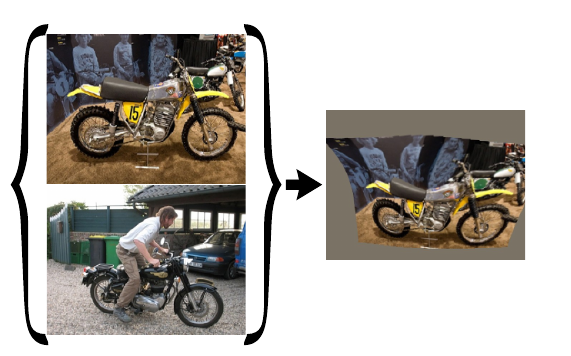
\includegraphics[scale=0.5]{images/Alignment}
  \caption{Trained geometry should
align two images with substantial appearance differences
}\label{fig:figure1}
\end{figure}      

	Recently, convolutional neural networks have been used to learn powerful feature descriptors which are more robust
	to appearance changes than the classical descriptors. However, these works still divide the image into
	a set of local patches and extract a descriptor individually from each patch. Extracted descriptors are then compared
	with an appropriate distance measure, by directly outputting a similarity score, or even by directly
	outputting a binary matching/non-matching decision. The paper which I am following had a different approach \cite{align}, treating the
	image as a whole, instead of a set of patches. Their approach has the advantage of capturing the interaction of the different
	parts of the image in a greater extent, which is not possible when the image is divided into a set of local regions

\end{itemize}
\begin{itemize}
	\item Deep Learning

	Deep learning aims to learn hierarchical feature representations by building high-level features from raw 
	data. In recent years, a variety of deep learning algorithms have been proposed in computer vision and machine
	learning and some of them have successfully applied to many visual analysis
	applications image classification, object detection, action recognition, face verification. Representative deep 
	learning methods include deep stacked auto-encoder \cite{34}, deep convolutional neural networks \cite{28}, and deep belief network \cite{17}.
	Deep learning has achieved great success in various visual applications including scalable image search. To my knowledge,
	Semantic hashing \cite{56} is the first work on using deep learning techniques to learn hashing functions for scalable
	image search. They applied the stacked Restricted Boltzmann Machine (RBM) learn compact binary codes for document
	search. However, their model is complex and requires pre training, which is not efficient for practical applications.

\end{itemize}

\end{document}
 
 
